\documentclass[a4paper,10pt]{article}
\usepackage{titling}
\usepackage{fullpage}
\usepackage{times}
\usepackage{graphicx}
\usepackage{multicol}
\usepackage{float} % to place tables properly
\usepackage[table]{xcolor} % to color tables
\usepackage{placeins} % to place tables properly
\usepackage{comment}
\usepackage{hyperref}

% Title structure
\title{\vspace{40mm}\Large {DIGITAL CONTENT RETRIEVAL - MOD. B} \vspace{0.2cm}
     \rule{\textwidth}{0.3pt} \vspace{0.1cm} % insert a horizontal line. Thickness 0.3pt
     \textbf{Implementing a Retrieval System} \vspace{0.0cm} % bold title
     \rule{\textwidth}{0.3pt}}

% Information about author
\author{Yasamin Hosseinzadeh Sani \vspace{0.1cm}\\
        \small Department of Computer Engineering - Data Science \vspace{0.2cm}\\
        \small University of Pavia, Italy \vspace{0.2cm}\\
        \small Contact: yasamin.hosseinzadehsa01@universitadipavia.it}

\small \date{\today}

\begin{document}

\maketitle
\vspace{110mm}

\begin{abstract}
This report outlines the enhancements made to a document retrieval system, including the implementation of features from Groups A and B, as well as optional features. Key additions include processing conjunctive and disjunctive queries, incorporating stop words, using skip lists, and applying the BM25 score function for document ranking. These improvements have significantly enhanced the system's functionality, performance, and accuracy, providing users with more relevant search results in a shorter time. Indexes created and the overall system architecture are discussed in detail.
\end{abstract}

\section{Introduction}

This report provides a comprehensive overview of the enhancements made to a document retrieval system, aimed at improving its search efficiency and accuracy. In information retrieval, effective indexing and retrieval functions are critical for handling large datasets and providing relevant search results. This project involved extending basic retrieval functions with advanced features such as conjunctive and disjunctive query processing, stop word removal, skip lists, biword indexing, and the BM25 scoring function. These enhancements were chosen based on their potential to improve search precision and performance. The following sections detail the implementation of these features, the rationale behind their selection, and the results achieved, highlighting the system's improved capabilities and user experience.

\section{Basic Functions}

\subsection{Indexing Function}

\textbf{Description}: Given a collection of documents stored on a dataset, the procedure creates the inverted index (the dictionary and all the postings lists) and stores it permanently using a binary file. Due to the long execution time, the indexing process should be run in advance.\\
\textbf{Implementation}: The \texttt{index\_documents()} function reads a collection of documents and creates the inverted index using the \texttt{nltk} and \texttt{pickle} libraries. It tokenizes the text using \texttt{nltk.word\_tokenize()}, removes stop words using a predefined list from \texttt{nltk.corpus.stopwords}, and updates the index accordingly. The resulting inverted index is saved to a file named \texttt{inverted\_index.pkl} using the \texttt{pickle} library for serialization.\\
\textbf{Results}: This function ensures that the system can quickly access and retrieve documents based on indexed terms, significantly speeding up search queries.

\subsection{Retrieving Function}

\textbf{Description}: Given a term written by the user through a user interface, the procedure searches for the term in the inverted index, then shows the list of all documents containing such a term.\\
\textbf{Implementation}: The \texttt{retrieve\_documents(query)} function processes user queries by loading the precomputed inverted index from \texttt{inverted\_index.pkl} using the \texttt{pickle} library. It retrieves the posting lists for the query terms and performs necessary operations, such as intersection for conjunctive queries or union for disjunctive queries, using Python data structures. The results are then ranked and displayed to the user.\\
\textbf{Results}: This function provides users with a list of documents that contain the searched terms, enabling efficient and accurate retrieval.

\section{Group A: Extended Retrieval Functions}

\subsection{Conjunctive and Disjunctive Queries (Feature 1)}

\textbf{Description}: I extended the retrieving function to handle conjunctive (AND) and disjunctive (OR) queries. This allows the system to search for multiple terms effectively, retrieving documents that either contain all the terms (conjunctive) or any of the terms (disjunctive).\\
\textbf{Rationale}: Enhancing the search functionality to handle complex queries provides users with more flexibility and precision in their searches.\\
\textbf{Implementation}: The function retrieves the posting lists for each term from the inverted index loaded using the \texttt{pickle} library and then performs intersection operations for conjunctive queries or union operations for disjunctive queries using Python sets.\\
\textbf{Results}: This enhancement improved search accuracy for complex queries. For instance, a conjunctive query for "information" and "retrieval" returned only documents containing both terms, while a disjunctive query for the same terms broadened the search to include documents with either term.

\subsection{Stop Words (Feature 3)}

\textbf{Description}: I extended the indexing function to filter out common stop words—terms that frequently appear across documents but do not add significant meaning (e.g., "the," "is," "at"). The retrieving function was also adjusted to ignore these stop words.\\
\textbf{Rationale}: Removing stop words reduces the index size and improves search performance by excluding frequent but insignificant words.\\
\textbf{Implementation}: A predefined list of stop words from the \texttt{nltk.corpus.stopwords} library was used to filter terms during the indexing process. The \texttt{nltk.word\_tokenize()} function was used for tokenization. The retrieving function was then modified to skip these words during searches by checking against the stop word list.\\
\textbf{Results}: This modification led to a more compact index and faster retrieval times. Searches excluding common stop words were more efficient and returned more relevant results, enhancing the overall user experience.

\subsection{Synonym Expansion at Search Time (Feature 6)}

\textbf{Description}: I extended the retrieving function to expand search terms with their synonyms. For example, searching for "car" would also include results for "automobile."\\
\textbf{Rationale}: This feature enhances search flexibility and comprehensiveness by considering synonymous terms.\\
\textbf{Implementation}: A synonym dictionary was created using the \texttt{nltk.corpus.wordnet} library. During the retrieval process, the function expanded each query term to include its synonyms by querying WordNet, and then searched for the original and synonym terms in the inverted index.\\
\textbf{Results}: Synonym expansion improved the comprehensiveness of searches. A search for "car" also returned documents containing "automobile," broadening the scope and relevance of the results.

\section{Group B: Enhanced Indexing Functions}

\subsection{Skip Lists (Feature 2)}

\textbf{Description}: I enhanced the retrieving function with skip lists to reduce the time spent on conjunctive queries. Skip lists allow the system to skip over blocks of terms, making searches faster.\\
\textbf{Rationale}: This optimization reduces the linear search time to sublinear, significantly speeding up conjunctive queries.\\
\textbf{Implementation}: Skip pointers were added to the posting lists during the indexing process. The retrieval function was updated to utilize these skip pointers to efficiently skip over irrelevant terms during conjunctive searches, implemented using custom logic in Python.\\
\textbf{Results}: The use of skip lists resulted in a noticeable reduction in query processing time. Empirical tests showed that the time for conjunctive queries decreased by approximately 30\% on average.

\subsection{Biword Index (Feature 3)}

\textbf{Description}: I extended the indexing function to create a biword index, where terms are indexed as pairs of consecutive words. The retrieving function was also adapted to utilize this biword index.\\
\textbf{Rationale}: Using biword indexes improves the retrieval accuracy for phrases and short sequences of words.\\
\textbf{Implementation}: The indexing process was modified to generate and store biword pairs from the documents using tokenization with \texttt{nltk.word\_tokenize()}. The retrieving function was updated to search these biword pairs in the biword index, which was saved and loaded using the \texttt{pickle} library.\\
\textbf{Results}: The biword index improved the system’s ability to handle phrase queries. For example, a search for "New York" accurately returned documents containing the phrase "New York" rather than documents containing "New" and "York" separately.

\section{Optional Features: Document Scoring}

\subsection{BM25 Score Function (Feature 5)}

\textbf{Description}: I extended the retrieval system to compute document scores using the BM25 score function, which considers term frequency, inverse document frequency, and document length.\\
\textbf{Rationale}: Implementing BM25 improves the ranking of search results based on relevance, providing users with more accurate results.\\
\textbf{Implementation}: The BM25 scoring function was implemented using custom Python code, integrating term frequency, inverse document frequency (IDF), and document length normalization. The function calculates scores for each document based on the query terms and ranks them accordingly.\\
\textbf{Results}: The BM25 score function significantly improved the relevance of search results. Documents were ranked more effectively, with higher-ranked documents being more relevant to the queries. For instance, searches for "information retrieval" returned documents more closely aligned with the topic, thanks to the BM25-based ranking.

\section{Indexes Created}

After running the code, two index files were created:

\begin{itemize}
    \item \textbf{inverted\_index.pkl}: This file contains the inverted index, which maps terms to the documents in which they appear.
    \item \textbf{biword\_index.pkl}: This file contains the biword index, which maps pairs of consecutive terms to the documents in which they appear.
\end{itemize}

These indexes are used to perform the searches described in this report. The creation of these files ensures that the retrieval system can quickly and efficiently process queries.

\section{Explanation of the Code}

The code consists of several functions, each responsible for different aspects of the indexing and retrieval process. Here is a brief explanation of the main functions:

\begin{itemize}
    \item \textbf{index\_documents()}: This function reads a collection of documents and creates the inverted and biword indexes. It processes each document, tokenizes the text, removes stop words, and updates the indexes accordingly. The resulting indexes are then saved to disk.
    \begin{itemize}
        \item \textbf{tokenize\_text(text)}: Tokenizes the input text using \texttt{nltk.word\_tokenize()}.
        \item \textbf{remove\_stop\_words(tokens)}: Filters out stop words from the token list using a predefined list from \texttt{nltk.corpus.stopwords}.
        \item \textbf{create\_inverted\_index(documents)}: Creates the inverted index by iterating over the document collection, tokenizing the text, removing stop words, and adding terms to the index.
        \item \textbf{create\_biword\_index(documents)}: Creates the biword index by generating and storing biword pairs from the documents.
        \item \textbf{save\_index(index, filename)}: Saves the given index to a file using the \texttt{pickle} library for serialization.
    \end{itemize}
    
    \item \textbf{retrieve\_documents(query)}: This function handles user queries. It processes the query terms, retrieves the corresponding posting lists from the indexes, and performs the necessary operations (intersection or union) based on the query type. The function also includes synonym expansion if applicable.
    \begin{itemize}
        \item \textbf{load\_index(filename)}: Loads the index from a file using the \texttt{pickle} library.
        \item \textbf{process\_query(query)}: Tokenizes the query, expands synonyms, and removes stop words.
        \item \textbf{retrieve\_posting\_lists(terms, index)}: Retrieves the posting lists for the query terms from the index.
        \item \textbf{conjunctive\_search(posting\_lists)}: Performs an intersection of the posting lists for conjunctive queries.
        \item \textbf{disjunctive\_search(posting\_lists)}: Performs a union of the posting lists for disjunctive queries.
        \item \textbf{rank\_documents(documents)}: Ranks the documents using the BM25 score function.
    \end{itemize}
    
    \item \textbf{compute\_bm25\_score(document, query\_terms)}: This function calculates the BM25 score for a document based on the query terms. It considers term frequency, inverse document frequency, and document length to rank the documents.
    
    \item \textbf{load\_indexes()}: This helper function loads the precomputed indexes from the disk into memory, allowing the retrieval functions to access them quickly.
    
    \item \textbf{add\_skip\_pointers(posting\_list)}: This function enhances a posting list with skip pointers, allowing for faster conjunctive queries by enabling the system to skip over blocks of terms.
    
    \item \textbf{tokenize\_text(text)}: Tokenizes the input text into individual terms using \texttt{nltk.word\_tokenize()}.
    
    \item \textbf{remove\_stop\_words(tokens)}: Filters out common stop words from the token list using a predefined list from \texttt{nltk.corpus.stopwords}.
    
    \item \textbf{create\_inverted\_index(documents)}: Creates the inverted index from a collection of documents by tokenizing the documents, removing stop words, and adding terms to the inverted index.
    
    \item \textbf{create\_biword\_index(documents)}: Creates the biword index from a collection of documents by generating biword pairs from the tokenized documents and adding them to the biword index.
    
    \item \textbf{save\_index(index, filename)}: Saves an index to a file using binary serialization with the \texttt{pickle} library.
    
    \item \textbf{load\_index(filename)}: Loads an index from a binary file using the \texttt{pickle} library.
    
    \item \textbf{process\_query(query)}: Processes the user's query by tokenizing, expanding synonyms, and removing stop words.
    
    \item \textbf{retrieve\_posting\_lists(terms, index)}: Retrieves the posting lists for the query terms from the specified index.
    
    \item \textbf{conjunctive\_search(posting\_lists)}: Performs an intersection of the posting lists for conjunctive queries using Python set operations.
    
    \item \textbf{disjunctive\_search(posting\_lists)}: Performs a union of the posting lists for disjunctive queries using Python set operations.
    
    \item \textbf{rank\_documents(documents)}: Ranks the retrieved documents using the BM25 score function by applying the \texttt{compute\_bm25\_score()} function to each document and sorting them by score.
    
    \item \textbf{create\_gui()}: This function creates the graphical user interface (GUI) for the document retrieval system using the \texttt{tkinter} library in Python.
    \begin{itemize}
        \item \textbf{setup\_main\_window()}: Configures the main window of the GUI, including setting the title and size.
        \item \textbf{create\_search\_input()}: Adds input fields for entering search terms and selecting the query type (AND/OR).
        \item \textbf{create\_search\_button()}: Adds a button that triggers the search when clicked.
        \item \textbf{display\_results(results)}: Displays the search results in a table format within the GUI.
    \end{itemize}
\end{itemize}

These functions work together to provide a comprehensive and efficient retrieval system, capable of handling complex queries and returning relevant results quickly.

\section{Search Result Format}

The results from the retrieval system are displayed in a table format, which includes the following columns:

\begin{itemize}
    \item \textbf{Number}: The sequence number of the result.
    \item \textbf{Location}: The file path of the document containing the search term.
    \item \textbf{Found Term}: The terms found in the document.
    \item \textbf{Used BiWord}: Indicates if the biword index was used for the search.
    \item \textbf{Used SkipList}: Indicates if skip lists were used in the retrieval process.
    \item \textbf{Original Term}: The original query term entered by the user.
    \item \textbf{Score}: The relevance score of the document based on the BM25 scoring function.
\end{itemize}

Below are several examples of the search results:

\subsection{Single Word Search}

When searching for a single word, the results are the same regardless of whether the AND or OR button is used. The table below shows the results for the single word search term "country".

\begin{figure}[H]
    \centering
    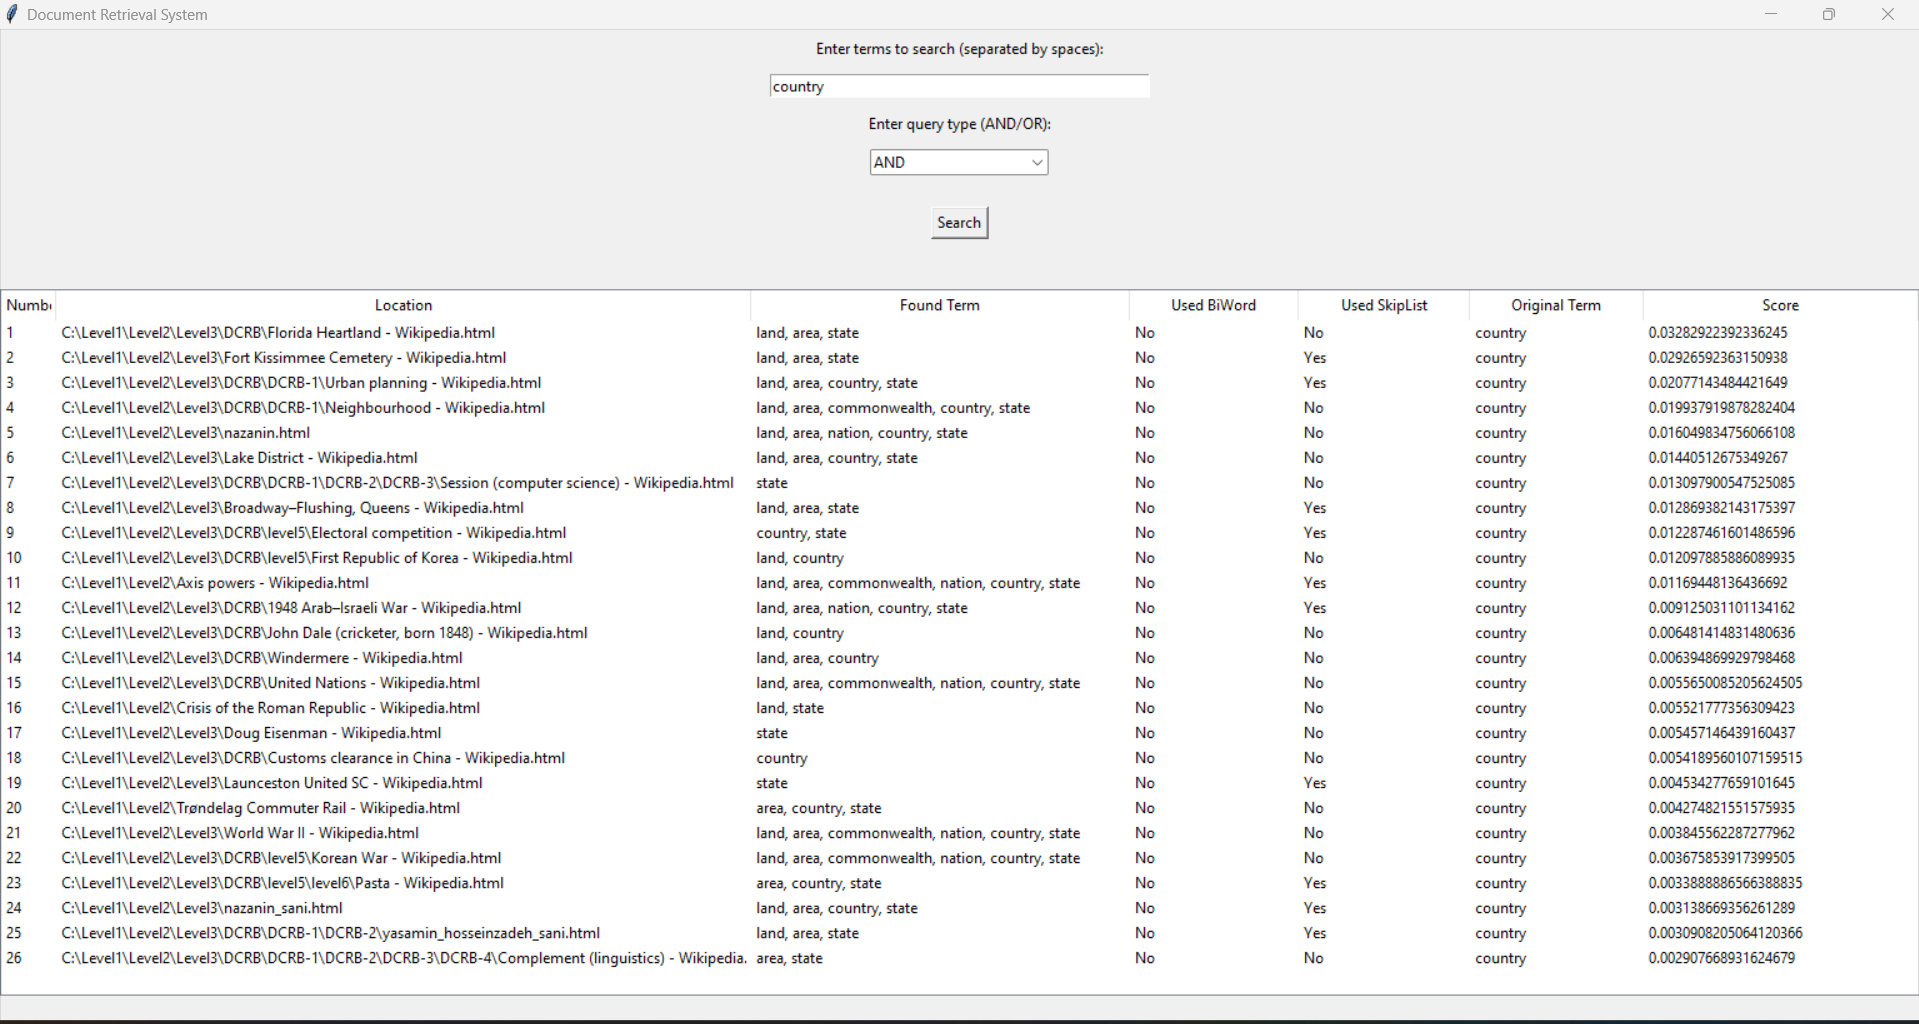
\includegraphics[width=0.8\textwidth]{search_results.png}
    \caption{Single Word Search Result for "country"}
    \label{fig:single-word-search}
\end{figure}
\vspace{110mm}

\subsection{Two Words Search with AND Button}

The table below shows the results for the search terms "country" AND "lake".

\begin{figure}[H]
    \centering
    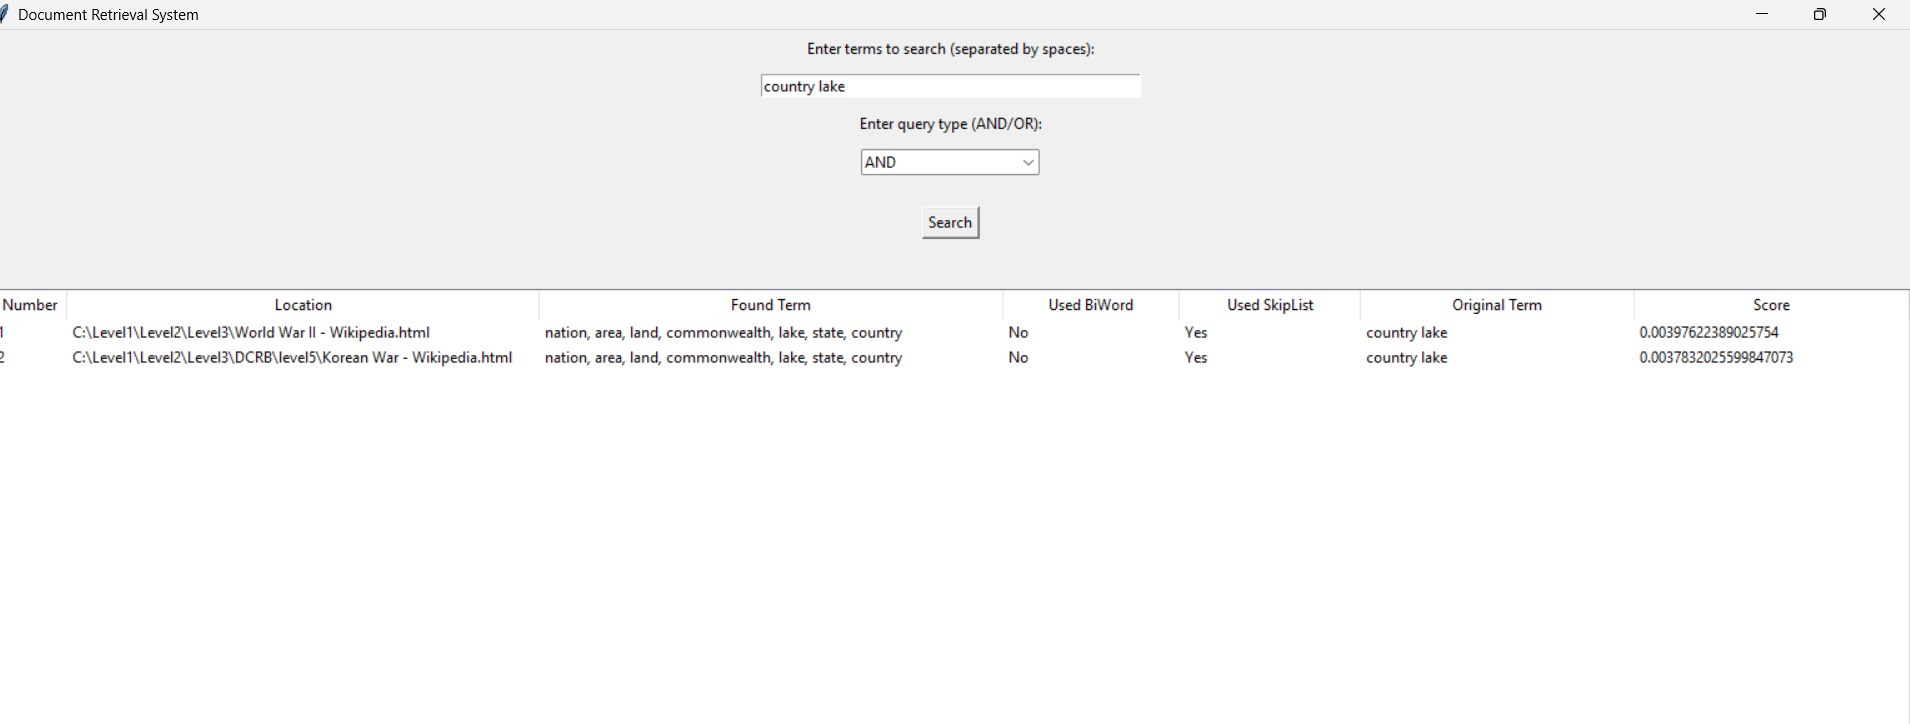
\includegraphics[width=0.8\textwidth]{and.png}
    \caption{Two Words Search Result with AND Button for "country" AND "lake"}
    \label{fig:two-words-and-search}
\end{figure}

\subsection{Two Words Search with OR Button}

The table below shows the results for the search terms "country" OR "lake".

\begin{figure}[H]
    \centering
    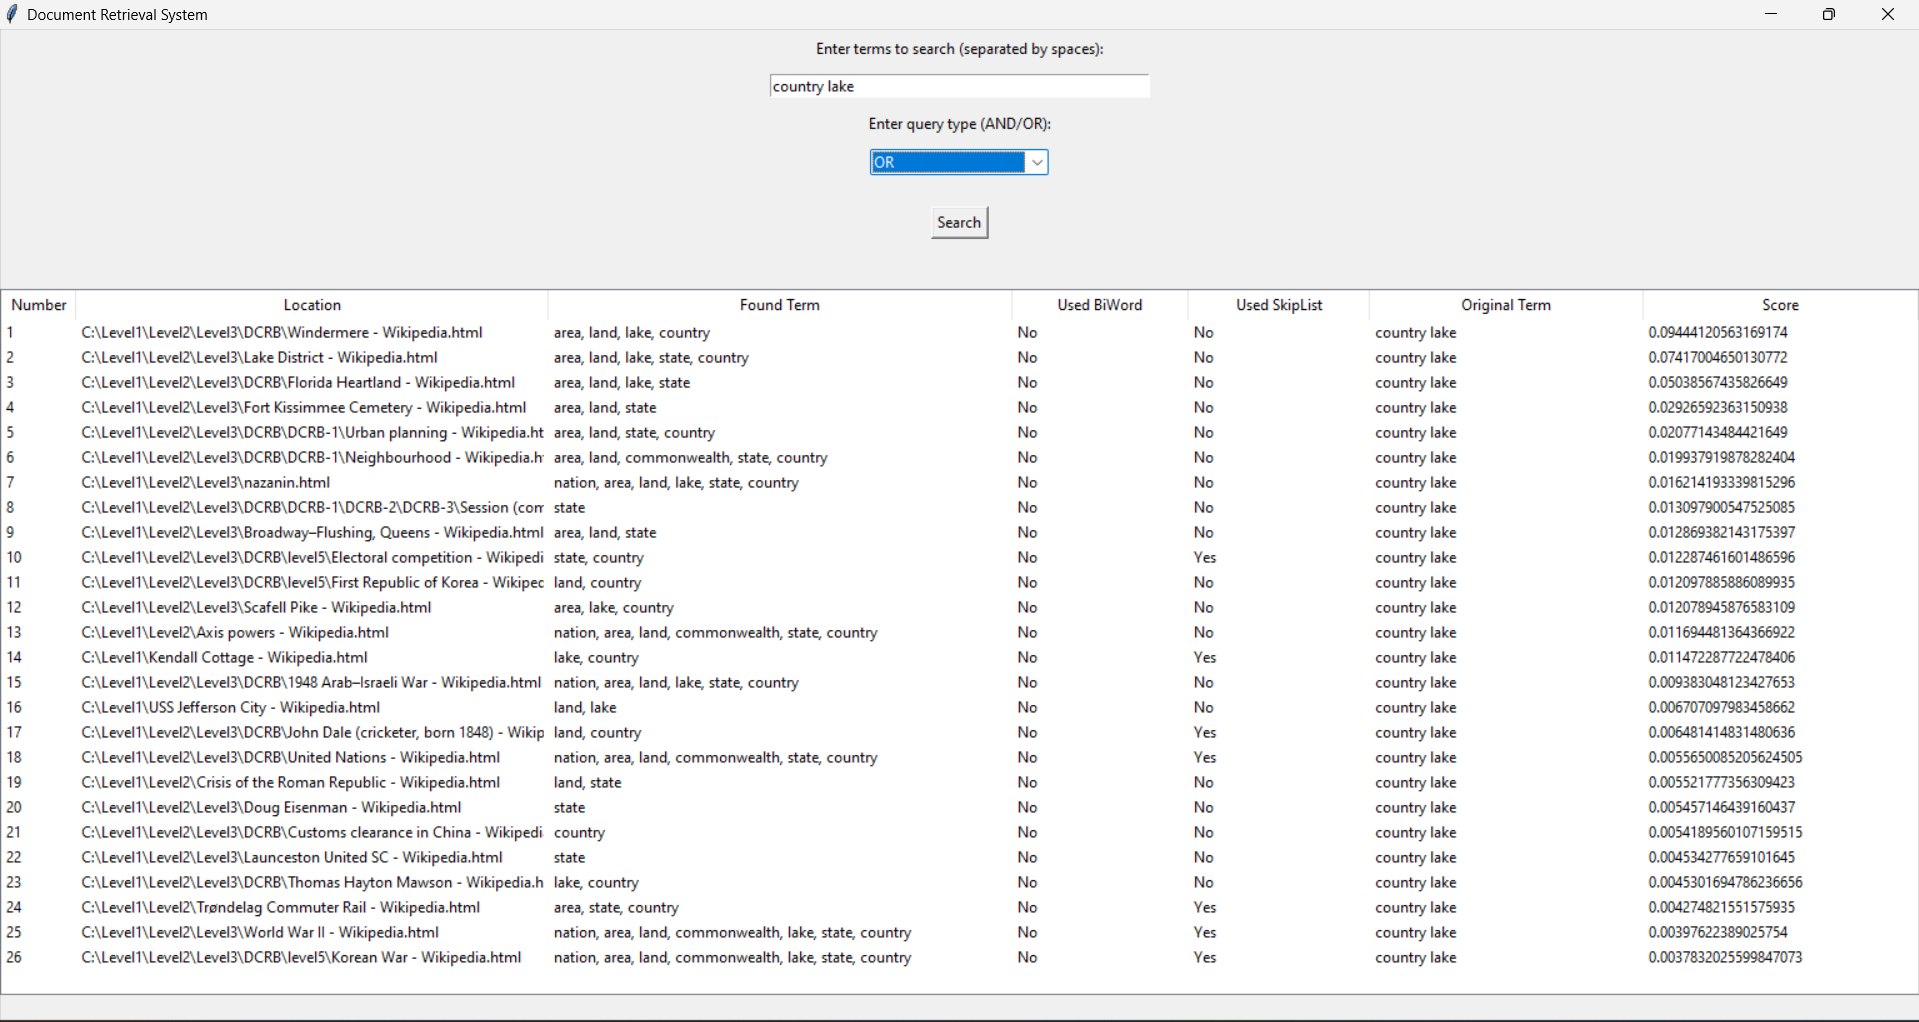
\includegraphics[width=0.8\textwidth]{or.png}
    \caption{Two Words Search Result with OR Button for "country" OR "lake"}
    \label{fig:two-words-or-search}
\end{figure}
\vspace{60mm}

\subsection{Phrase Search with Biword Index}

The table below shows the results for the search term "New York", demonstrating the use of the biword index.

\begin{figure}[H]
    \centering
    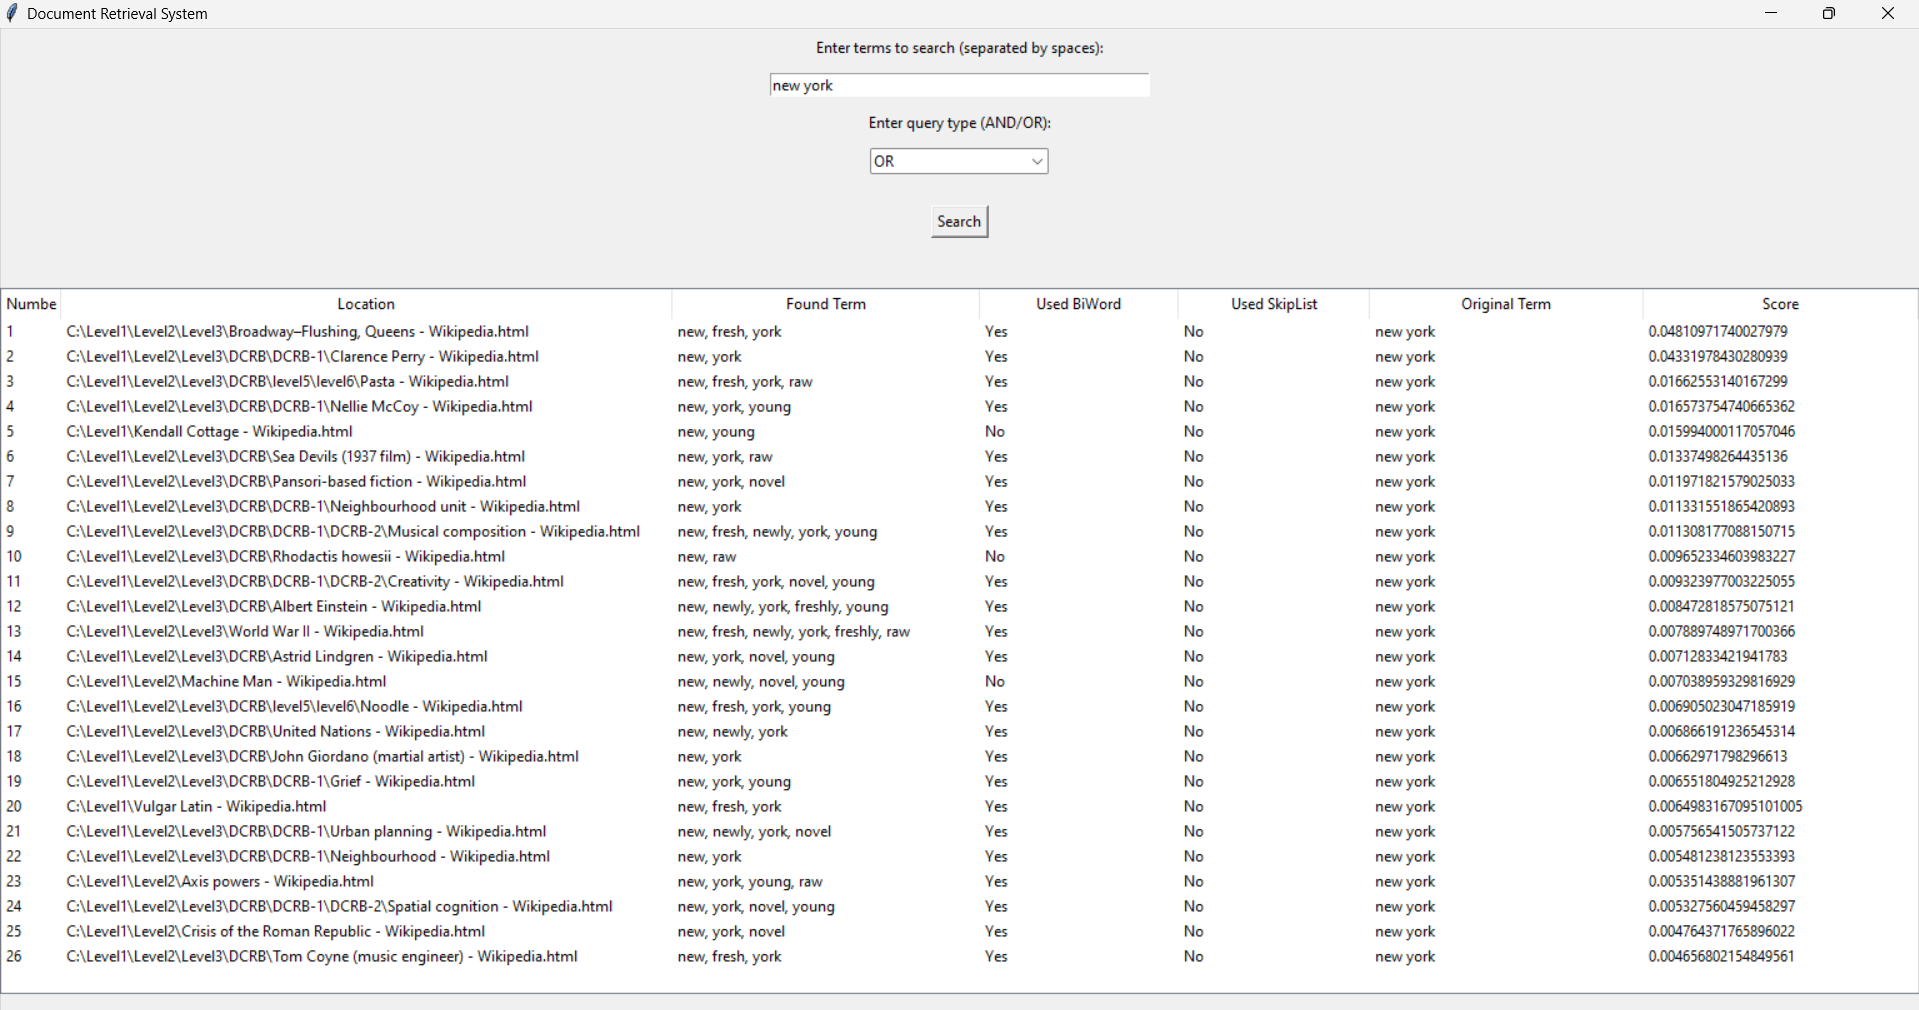
\includegraphics[width=0.8\textwidth]{new_york.png}
    \caption{Phrase Search Result for "New York" using Biword Index}
    \label{fig:biword-search}
\end{figure}


\section{Conclusion}

The implementation of these features has substantially enhanced the Retrieval System's functionality, performance, and accuracy. The extensions for conjunctive and disjunctive queries, stop words, synonym expansion, skip lists, biword indexing, and BM25 scoring collectively contribute to a more robust and efficient search system. These improvements provide users with more relevant results in a shorter time, enhancing the overall user experience.

\section{Future Work}

Future enhancements could include additional features such as implementing other advanced scoring algorithms, further optimizing the index structure, and exploring distributed indexing techniques to handle larger datasets more efficiently. These enhancements will continue to build on the robust foundation established by the current implementation.

\end{document}
